\documentclass[fullscreen=true, bookmarks=true, hyperref={pdfencoding=unicode}]{beamer}
\usepackage[utf8]{inputenc}                                % Кодировка
\usepackage[english,russian]{babel}                        % Переносы
\usepackage{xcolor}                                        % Работа с цветом
\usepackage{amsmath,amssymb,amsfonts}                      % Символы АМО
\usepackage{graphicx}                                      % Графика
\usepackage[labelsep=period]{caption}                      % Разделитель в подписях к рисункам и таблицам
\usepackage{hhline}                                        % Для верстки линий в таблицах
\usepackage{tikz}                                          % Для простых рисунков в документе
\usepackage{fancybox}                                      % Пакет для отрисовки рамок
\usepackage{verbatim}                                      % Для вставки кода в презентацию
\usepackage{animate}                                       % Для вставки видео в презентацию
\usepackage{xmpmulti}                                      % Для вставки gif в презентацию
\usepackage{multirow}
\usepackage{mathrsfs}

\usetikzlibrary{arrows, snakes, backgrounds}                 % Для отрисовки стрелок
\usetikzlibrary{positioning, fit, arrows.meta, shapes, calc}
% used to avoid putting the same thing several times...
% Command \empt{var1}{var2}
\newcommand{\empt}[2]{$#1^{\langle #2 \rangle}$}

\graphicspath{{images/}}                                   % Путь до рисунков
\setbeamertemplate{caption}[numbered]                      % Включение нумерации рисунков

\definecolor{links}{HTML}{2A1B81}                          % blue for url links
\hypersetup{colorlinks,linkcolor=,urlcolor=links}          % nothing for others

\usetheme{boxes}
\usecolortheme{crane}

\usepackage{pythonhighlight}

\newtheorem*{question}{Вопрос}

\title{Лекция 6. Тематическое моделирование и word2vec}
\author{Александр Юрьевич Авдюшенко}
\institute{МКН СПбГУ}
\date{24 марта 2022}
\titlegraphic{
\includegraphics[keepaspectratio,width=0.5\textwidth]{logo_fmkn.png}}

\begin{document}
%\unitlength=2mm

% выводим заглавие
\begin{frame}
\transdissolve[duration=0.2]
\titlepage
\end{frame}


\begin{frame}
  \frametitle{Пятиминутка}
  \begin{itemize}
    \item Какие основные недостатки архитектуры encoder-decoder?
    \item Выпишите формулу модели внимания $Attn(q,K,V)$
    \item Опишите два критерия для обучения BERT
  \end{itemize}
\end{frame}


\begin{frame}
  \frametitle{План лекции}
  \begin{enumerate}
    \item тематическое моделирование
    \begin{itemize}
      \item Probabilistic latent semantic analysis (PLSA) и ARTM
      \item Latent Dirichlet Allocation (LDA)
      \item регуляризаторы ARTM
      \item метрики качества
    \end{itemize}
    \item word2vec
    \end{enumerate}
\end{frame}


\begin{frame}
  \frametitle{Возможные определения}

  Тема —
  \begin{enumerate}
    \item специальная терминология предметной области
    \item набор часто совместно встречающихся терминов
    \item семантически однородный кластер текстов
  \end{enumerate}
\end{frame}


\begin{frame}
  \begin{center}
    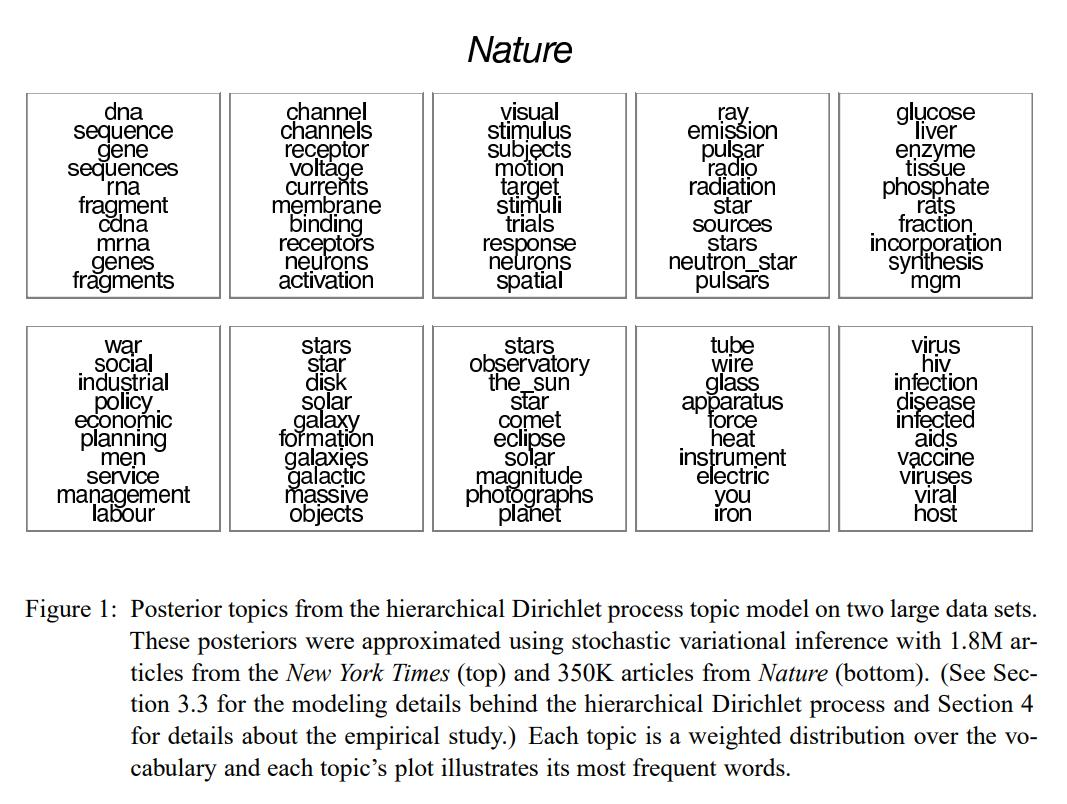
\includegraphics[keepaspectratio,
                   width=.7\paperwidth]{nature_topics.jpg}
  \end{center}

  \noindent\rule{8cm}{0.4pt}

  {\small
  {\it Matthew D. Hoffman , David M. Blei, Chong Wang, John Paisley}. Stochastic Variational Inference, \href{https://arxiv.org/abs/1206.7051}{https://arxiv.org/abs/1206.7051}}
\end{frame}


\begin{frame}
  \frametitle{Сферы применения тематического моделирования}

  \begin{itemize}
    \item анализ и агрегирование новостных потоков
    \item рубрикация документов, изображений, видео, музыки
    \item рекомендательные сервисы
    \item поиск экспертов, рецензентов или проектов
    \item выявление трендов и фронтов исследований
  \end{itemize}
\end{frame}


\begin{frame}
  \frametitle{Математическое определение темы}

  \begin{itemize}
    \item Тема — условное дискретное вероятностное распределение на множестве терминов

          $\color{red}{p(w | t)}$ — вероятность термина $w$ в теме $t$

    \item Тематический профиль документа — условное распределение

          $\color{red}{p(t | d)}$ — вероятность темы $t$ в документе $d$
  \end{itemize}
\end{frame}

\begin{frame}
  \frametitle{Порождающая модель}

  $W$ — конечное множество слов (терминов, токенов)

  $D$ — конечное множество текстовых документов

  $T$ — конечное множество тем

  $W \times D \times T$ — дискретное вероятностное пространство

  \pause
  \vspace{1cm}
  \begin{block}{Гипотезы}
    \begin{itemize}
      \item порядок слов в документе не важен (bag of words)

            Коллекция — это выборка $(w_i, d_i, t_i)_{i=1}^n \sim p(w, d, t)$

      \item гипотеза условной независимости: $p(w|d, t) = p(w|t)$

            $ p(w|d) = \sum\limits_{t\in T}p(t|d)p(w|t)$
    \end{itemize}
  \end{block}
\end{frame}


{ % all template changes are local to this group.
    \setbeamertemplate{navigation symbols}{}
    \begin{frame}<article:0>[plain]
        \begin{tikzpicture}[remember picture,overlay]
            \node[at=(current page.center)] {
                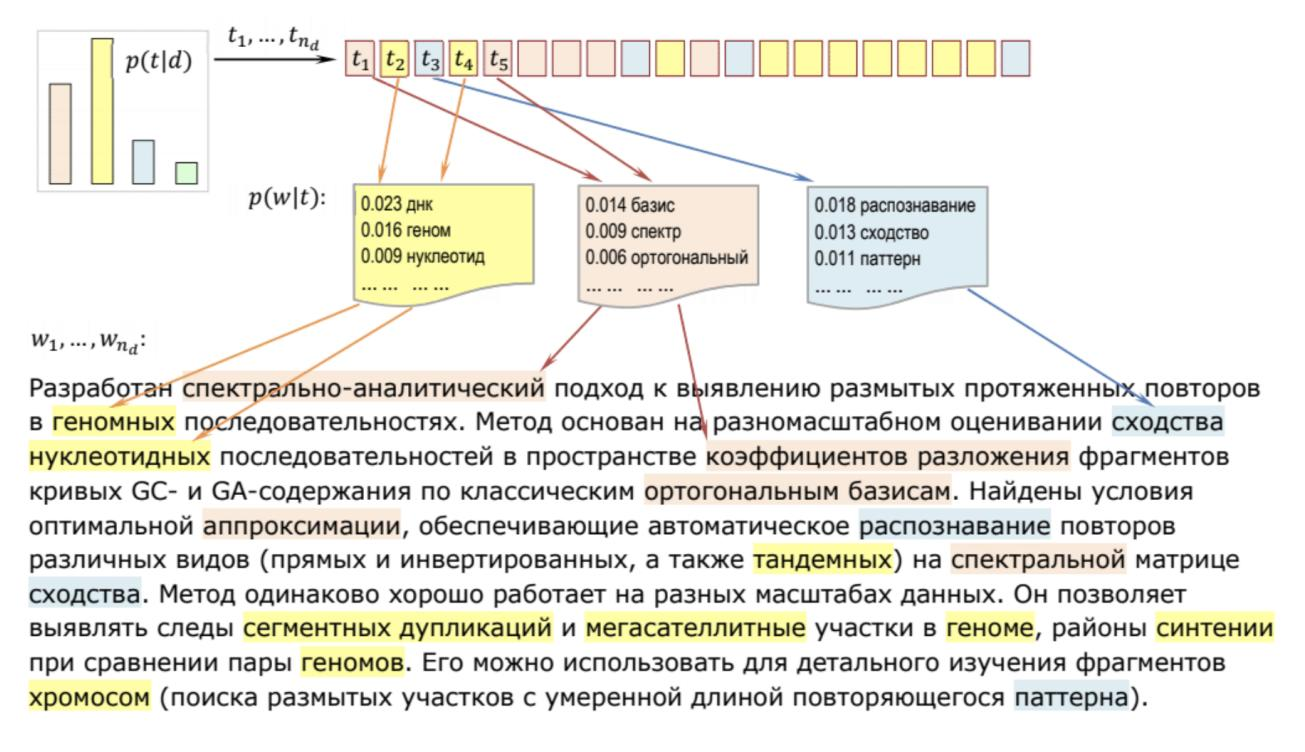
\includegraphics[keepaspectratio,
                                 width=\paperwidth,
                                 height=\paperheight]{doc_generation.jpg}
            };
        \end{tikzpicture}
     \end{frame}
}


\begin{frame}
  \frametitle{Обратная задача}

  {\bf Дано}: коллекция текстовых документов

  \begin{itemize}
    \item $n_{dw}$ — частоты терминов в документах,  $\hat p (w | d) = \frac{n_{dw}}{n_{d}}$
  \end{itemize}

  {\bf Найти}: параметры тематической модели  $p(w|d) = \sum\limits_{t \in T} \phi_{wt} \theta_{td}$

  \begin{itemize}
    \item $\phi_{wt} = p(w|t)$ — вероятности терминов $w$ в каждой теме $t$
    \item $\theta_{td} = p(t|d)$ — вероятности тем $t$ в каждом документе $d$
  \end{itemize}

  \begin{center}
    Это задача стохастического матричного разложения
    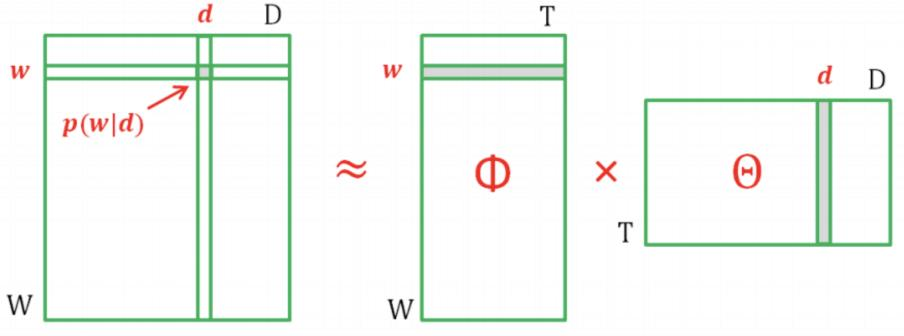
\includegraphics[keepaspectratio,
                     width=.6\paperwidth]{matrix_decomposition.jpg}
  \end{center}
\end{frame}


\begin{frame}
  \frametitle{Принцип максимума правдоподобия}

  {\bf Правдоподобие} — плотность распределения выборки $(d_i, w_i)_{i=1}^n$:

  $$\prod\limits_{i=1}^n p(d_i, w_i) = \prod\limits_{d \in D} \prod\limits_{w \in d} p(d, w)^{n_{dw}} $$

  {\bf Максимизация логарифма правдоподобия}

  $$\sum\limits_{d \in D} \sum\limits_{w \in d} n_{dw} \ln{\color{red}p(w|d)}{\color{gray}p(d)} \to \max\limits_{\Phi, \Theta} $$

  приводит к задаче математического программирования:

  $$\sum\limits_{d \in D} \sum\limits_{w \in d} n_{dw} \ln{\color{red}\sum\limits_{t\in T} \phi_{wt}\theta_{td}} \to \max\limits_{\Phi, \Theta} $$

  при ограничениях неотрицательности и нормировки:

  \begin{align*}
    \phi_{wt} &\geq 0, \sum\limits_{w \in W}\phi_{wt} = 1, \\
    \theta_{td} &\geq 0, \sum\limits_{t \in T}\theta_{wt} = 1
  \end{align*}
 \end{frame}


\begin{frame}
  \frametitle{Бесконечность решений задачи}

  Задача матричного разложения {\bf некорректно поставлена}:

  если $\Phi, \Theta$ — решение, то стохастические $\Phi^\prime, \Theta^\prime$ — тоже решения

  \begin{itemize}
    \item $\Phi^\prime\Theta^\prime = (\Phi S)(S^{-1}\Theta), rank S = |T|$
    \item $\mathcal{L}(\Phi^\prime, \Theta^\prime) = \mathcal{L}(\Phi, \Theta)$
    \item $\mathcal{L}(\Phi^\prime, \Theta^\prime) \leq \mathcal{L}(\Phi, \Theta) + \varepsilon$ — приближённые решения
  \end{itemize}

  \vspace{1cm}
  {\bf Регуляризация} — стандартный приём доопределения решения с помощью дополнительных критериев
\end{frame}


\begin{frame}
  \frametitle{Приницип максимума правдоподобия (PLSA и ARTM)}

  Максимизация логарифма правдоподобия {\color{red}с регуляризатором}:

  $$\sum\limits_{d, w} n_{dw} \ln {\sum\limits_{t\in T} \phi_{wt}\theta_{td}} +{\color{red} R(\Phi, \Theta)} \to \max\limits_{\Phi, \Theta} $$

  EM-алгоритм: метод простой итерации для системы уравнений
  $$ \begin{array}{c}
   E-\text{шаг} \\ \\ \\ M-\text{шаг}
  \end{array}
  \begin{cases}
      p_{tdw} \equiv p(t|d,w) = \underset{t \in T}{\text{norm}}(\phi_{wt}\theta_{td}) \\
      \phi_{wt} = \underset{w \in W}{\text{norm}}\left(n_{wt} +{\color{red} \phi_{wt} \frac{\partial R}{\partial \phi_{wt}}} \right), \quad n_{wt} = \sum\limits_{d\in D} n_{dw} p_{tdw} \\
      \theta_{td} = \underset{t \in T}{\text{norm}}\left(n_{td} +{\color{red} \theta_{td} \frac{\partial R}{\partial \theta_{td}}} \right), \quad n_{td} = \sum\limits_{w\in d} n_{dw} p_{tdw}
    \end{cases}
  $$

  где $\underset{t \in T}{\text{norm}}\left(x_t\right) = \frac{\max(x_t, 0)}{\sum\limits_{s \in T}\max(x_s, 0)}$ — операция нормировки вектора

  Если $R(\Phi, \Theta) = 0$, то перед нами {\bf Probabilistic latent semantic analysis (PLSA)}. Если нет, то {\bf адаптивная регуляризация тематических моделей (ARTM)}.
\end{frame}


\begin{frame}
  \frametitle{Вырожденность тем и документов}

  \begin{block}{{\it Тема} $t$ вырождена}
    Если для всех терминов $w \in W$

    $$ n_{wt} + \phi_{wt} \frac{\partial R}{\partial \phi_{wt}} \leq 0 $$
  \end{block}

  Если тема $t$ вырождена, то $p(w|t) = \phi_{wt} \equiv 0$

  \begin{block}{{\it Документ} $d$ вырожден}
    Если для всех тем $t \in T$

    $$ n_{td} + \theta_{td} \frac{\partial R}{\partial \theta_{td}} \leq 0 $$
  \end{block}

  Если документ $d$ вырожден, то $p(t|d) = \theta_{td} \equiv 0$
\end{frame}


\begin{frame}
  \frametitle{Latent Dirichlet Allocation (LDA)}

  \begin{center}
    Распределение на симплексе
    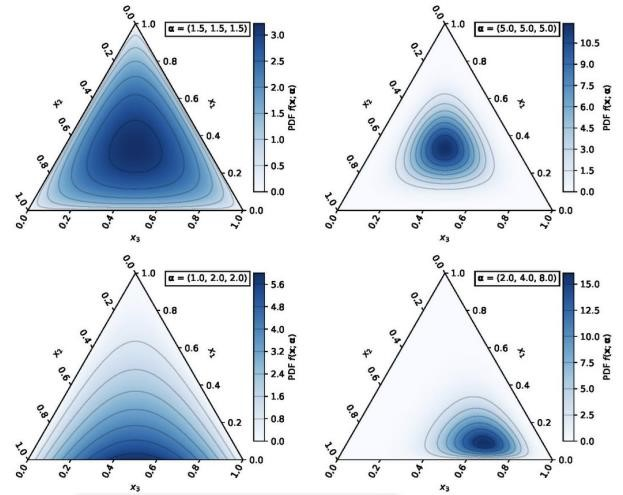
\includegraphics[keepaspectratio,
                     width=.7\paperwidth]{LDA.jpg}
  \end{center}
\end{frame}


{ % all template changes are local to this group.
    \setbeamertemplate{navigation symbols}{}
    \begin{frame}<article:0>[plain]
        \begin{tikzpicture}[remember picture,overlay]
            \node[at=(current page.center)] {
            \animategraphics[loop,width=.6\paperwidth,autoplay]{4}{LDA-}{0}{99}
            };
        \end{tikzpicture}
     \end{frame}
}


\begin{frame}
  \frametitle{Распределение Дирихле}

  {\bf Гипотеза}. Вектор-столбцы $\phi_t = (\phi_{wt})$ и $\theta_d = (\theta_{td})$ порождаются распределениями Дирихле с параметрами $\alpha \in \mathbb{R}^{|T|}, \beta \in \mathbb{R}^{|W|}$:

  $$\text{Dir}(\phi_t | \beta) = \frac{\Gamma(\sum\limits_w \beta_w)}{\prod\limits_w \Gamma(\beta_w)} \prod\limits_w \phi_{wt}^{\beta_w-1}, \quad \phi_{wt} > 0, \quad \beta_w > 0 $$

  $$\text{Dir}(\theta_d | \alpha) = \frac{\Gamma(\sum\limits_t \alpha_t)}{\prod\limits_t \Gamma(\alpha_t)} \prod\limits_t \theta_{td}^{\alpha_t-1}, \quad \theta_{td} > 0, \quad \alpha_t > 0 $$
\end{frame}


\begin{frame}
  \frametitle{Максимум апостериори}

  Совместное правдоподобие данных и модели

  $$ \ln \prod\limits_{d \in D}\prod\limits_{w \in d} p(w, d | \Phi, \Theta)^{n_{dw}}
     {\color{red}\prod\limits_{t \in T}\text{Dir}(\phi_t|\beta) \prod\limits_{d \in D} \text{Dir}(\theta_d | \alpha)} \to \max\limits_{\Phi, \Theta}$$

  Регуляризатор — логарифм априорного распределения:

  $$ R(\Phi, \Theta) = \sum\limits_{t, w} \left(\beta_w - 1\right) \ln \phi_{wt} + \sum\limits_{d, t} \left(\alpha_t - 1\right) \ln \theta_{td} $$

  M-шаг — сглаженные или разреженные частотные оценки:

  $$ \phi_{wt} = \underset{w \in W}{\text{norm}}\left(n_{wt} {\color{red}+ \beta_{w} -1} \right),
     \theta_{td} = \underset{t \in T}{\text{norm}}\left(n_{td} {\color{red}+ \alpha_{t} - 1} \right) $$

  при $\beta_w > 1, \alpha_t > 1$ — сглаживание,

  при $0 < \beta_w < 1, 0 < \alpha_t < 1$ — слабое разреживание
\end{frame}


\begin{frame}
  \frametitle{Преимущества распределения Дирихле}

  \begin{itemize}
    \item сопряженное к мультиномиальному
    \item как следствие, если априорное распределение обозначено как $\text{Dir}(\alpha)$, то $\text{Dir}(\alpha + \gamma)$ есть апостериорное распределение после серии наблюдений с гистограммой $\gamma$
    \item это очень удобно для байесовского вывода
    \item ещё можем управлять разреженностью через коэффициенты
  \end{itemize}
\end{frame}


\begin{frame}
  Группа К.В. Воронцова (библиотека ARTM) предложила просто эмпирически строить разные регуляризаторы, возможно без вероятностного обоснования.

  В нашем курсе подробно про это не будем, но вообще так можно
  \begin{itemize}
    \item строить модели мультимодального тематического моделирования (например, текст, картинка и время в каждом документе)
    \item решать задачи классификации, регрессии на документах одновременно с решением задачи выделения тем (не последовательно)
    \item выделять фоновые темы (содержащие слова общей лексики)
    \item усиливать различность тем
  \end{itemize}
\end{frame}


\begin{frame}
  \frametitle{Метрики качества в тематическом моделировании}
  \framesubtitle{Правдоподобие и перплексия (perplexity, implicit мера)}

  {\it Правдоподобие} языковой модели $p(w|d)$ — чем больше, тем лучше:
  $$ \mathcal{L} (\Phi, \Theta) = \sum\limits_{d \in D} \sum\limits_{w \in d} n_{dw} \ln p(w|d),
  \quad p(w|d) = \sum\limits_t \phi_{wt} \theta_{td}$$

  {\it Перплексия} языковой модели $p(w|d)$ — чем меньше, тем лучше:
  $$ \mathcal{P} (D) = \exp\left(-\frac{1}{n} \sum\limits_{d \in D} \sum\limits_{w \in d} n_{dw} \ln p(w|d) \right),
  \quad n = \sum\limits_{d \in D}\sum\limits_{w \in d} n_{dw}$$

 {\bf Интерпретация перплексии}:
 \begin{itemize}
   \item если распределение $p(w|d) = \frac{1}{|W|}$ равномерное, то $\mathcal{P} = |W|$
   \item мера различности или неопределённости слов в тексте
   \item коэффициент ветвления (branching factor) текста
 \end{itemize}
\end{frame}


\begin{frame}
  \frametitle{Перплексия тестовой (отложенной) выборки}

  {\it Перплексия} тестовой коллекции $D^\prime$ (hold-out perplexity):

  $$ \mathcal{P} (D^\prime) = \exp\left(-\frac{1}{n^{\prime\prime}} \sum\limits_{d \in D^{\prime}} \sum\limits_{w \in d^{\prime\prime}} n_{dw} \ln p(w|d) \right),
     \quad n^{\prime\prime} = \sum\limits_{d \in D^{\prime}}\sum\limits_{w \in d^{\prime\prime}} n_{dw}$$

  \begin{itemize}
    \item $d = d^{\prime}\cap d^{\prime\prime}$ — случайное разбиение тестового документа на две половины равной длины
    \item параметры $\phi_{wt}$ оцениваются по обучающей коллекции $D$
    \item параметры $\theta_{td}$ оцениваются по первой половине $d^\prime$
    \item перплексия вычисляется по второй половине $d^{\prime\prime}$
  \end{itemize}
\end{frame}


\begin{frame}
  \frametitle{Интерпретируемость}
  \framesubtitle{explicit мера}

  Экспертные оценки
  \begin{itemize}
    \item интерпретируемость темы по балльной шкале
    \item каждую тему оценивают несколько экспертов
  \end{itemize}
  \vspace{1cm}
  Метод интрузий (intrusion)
  \begin{itemize}
    \item в список топовых слов внедряется лишнее слово
    \item измеряется доля ошибок экспертов при его определении
  \end{itemize}

\end{frame}


\begin{frame}
  \frametitle{Когерентность}
  \framesubtitle{implicit мера}

  Когерентность (согласованность) темы $t$ по $k$ топовым словам:

  $$ \text{PMI}_t = \frac{2}{k(k-1)} \sum\limits_{i=1}^{k-1} \sum\limits_{j=i+1}^{k} \text{PMI}(w_i, w_j) $$

  где $w_i$ — $i$-й термин в порядке убывания $\phi_{wt}$

  \vspace{0.5cm}
  $\text{PMI}(u, v) = \ln \frac{|D|N_{uv}}{N_u N_v}$ — поточечная взаимная информация (pointwise mutual information)

  $N_{uv}$ — число документов, в которых термины $u, v$ хотя бы один раз встречаются рядом (в окне 10 слов)

  $N_{u}$ — число документов, в которых $u$ встретился хотя бы один раз

  \noindent\rule{8cm}{0.4pt}

  {\footnotesize
  {\it Newman D., Lau J.H., Grieser K., Baldwin T.} Automatic evaluation of topic coherence // Human Language Technologies, HLT-2010, Pp. 100-108.}
\end{frame}


{ % all template changes are local to this group.
    \setbeamertemplate{navigation symbols}{}
    \begin{frame}<article:0>[plain]
        \begin{tikzpicture}[remember picture,overlay]
            \node[at=(current page.center)] {
                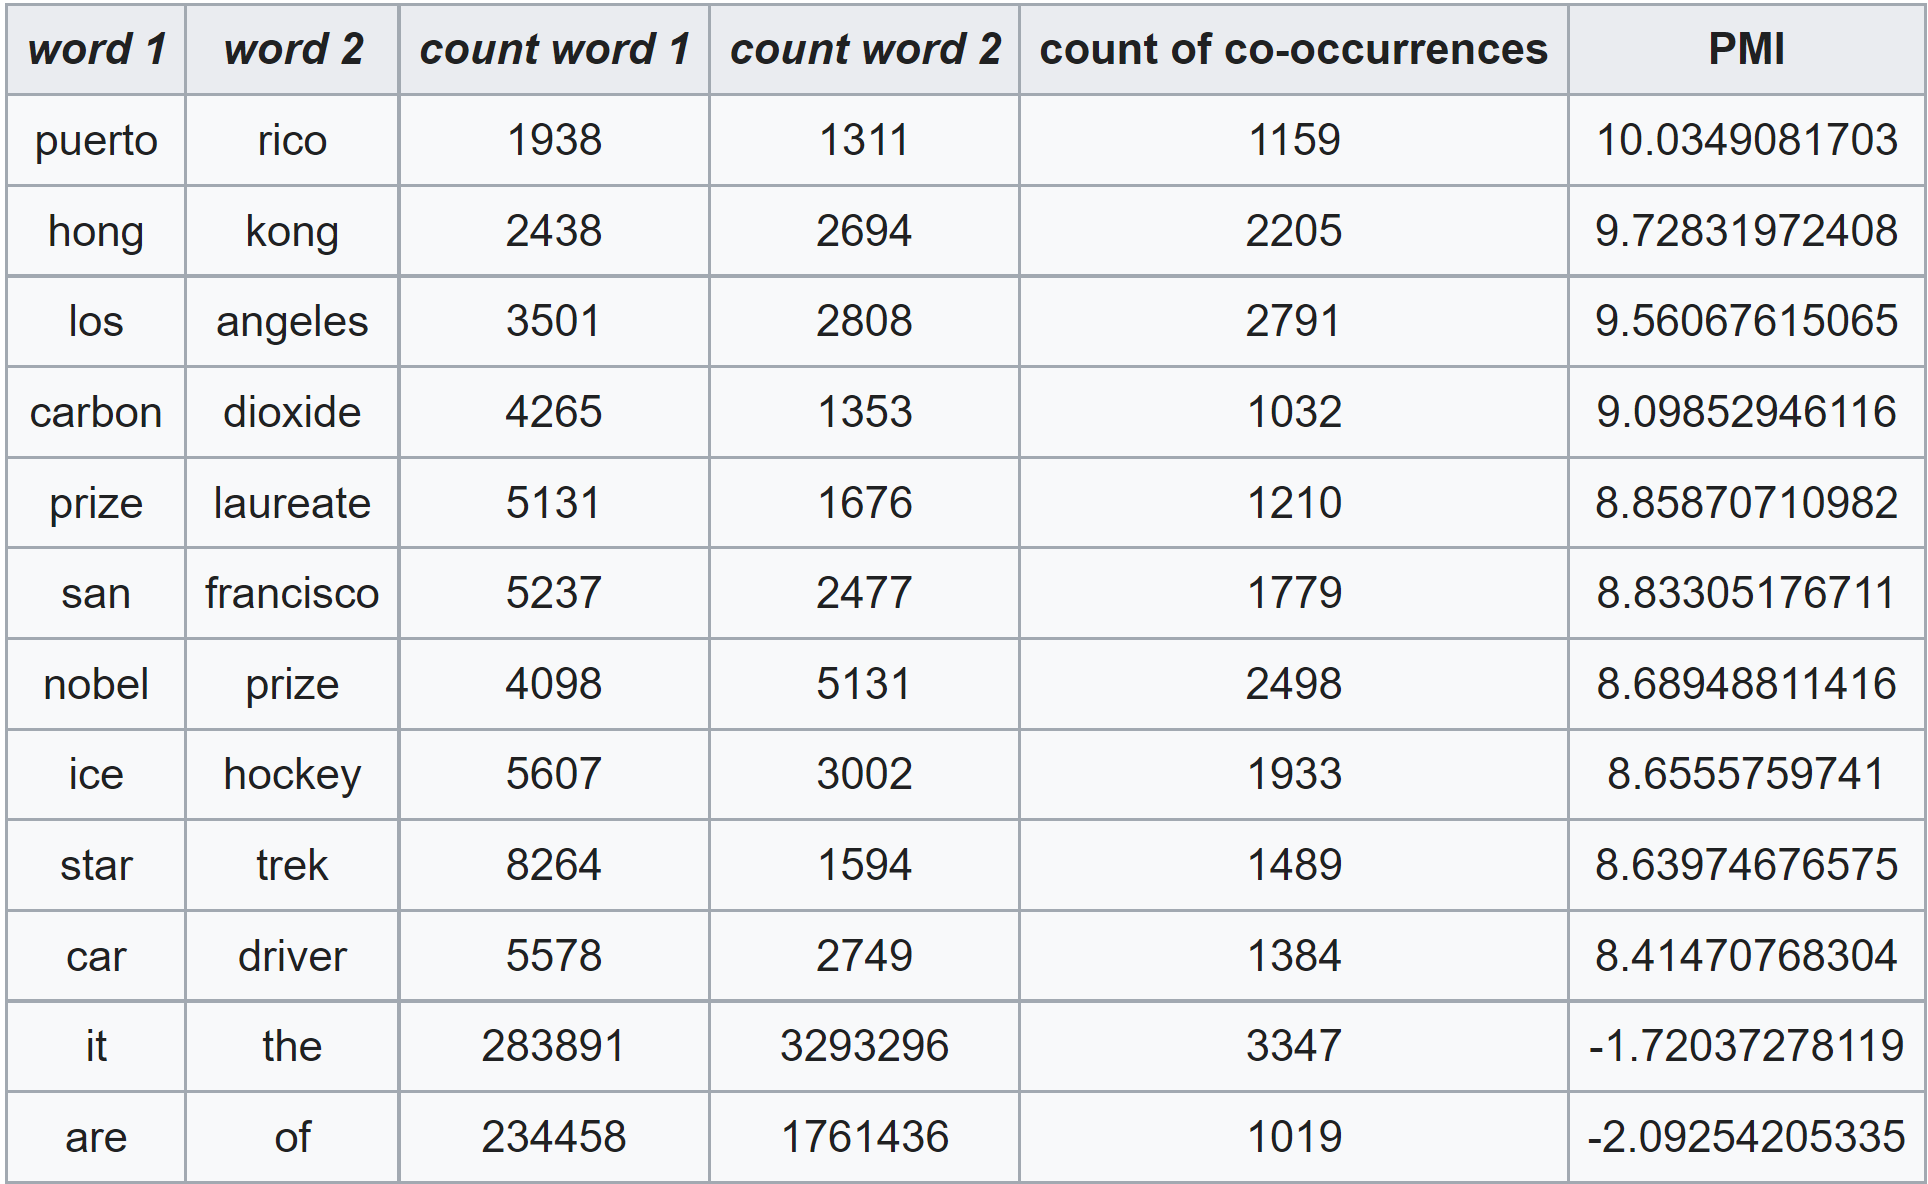
\includegraphics[keepaspectratio,
                                 width=\paperwidth,
                                 height=\paperheight]{wiki_pmi.png}
            };
        \end{tikzpicture}
     \end{frame}
}


\begin{frame}
  \frametitle{Word2Vec}
  \framesubtitle{Мотивация}

  One-hot encoding представления
  \begin{itemize}
    \item никак не отражают смысловую близость слов
    \item имеют слишком большую размерность
  \end{itemize}

  \vspace{1.5cm}
  Например,

  скалодром [0, 1, 0, 0, 0, 0]

  диван [0, 0, 1, 0, 0, 0]

  отдых [0, 0, 0, 1, 0, 0]
\end{frame}


\begin{frame}
  \frametitle{Идея — смотреть контекст}

  «You shall know a word by the company it keeps»

  (J.R. Firth, 1957)

  \vspace{1cm}
  Пример
  \begin{itemize}
    \item из всех домашних животных {\bf ???} лучше всего справляются с ловлей мышей
  \end{itemize}

\end{frame}


\begin{frame}
  \frametitle{Continuous Bag of Words (CBOW) and Skip-gram}
  \vspace{-.25cm}
  {\small
  \begin{align*}
    \frac{1}{T}\sum\limits_{t=1}^T \log(p(w_{t}|w_{t-m}, \dots, w_{t-1}, w_{t+1}, \dots, , w_{t+m})) \\
   \frac{1}{T}\sum\limits_{t=1}^T \sum\limits_{-m \leq j \leq m, j \neq 0} \log(p(w_{t-j}|w_{t}))
  \end{align*}
  }

  \begin{center}
    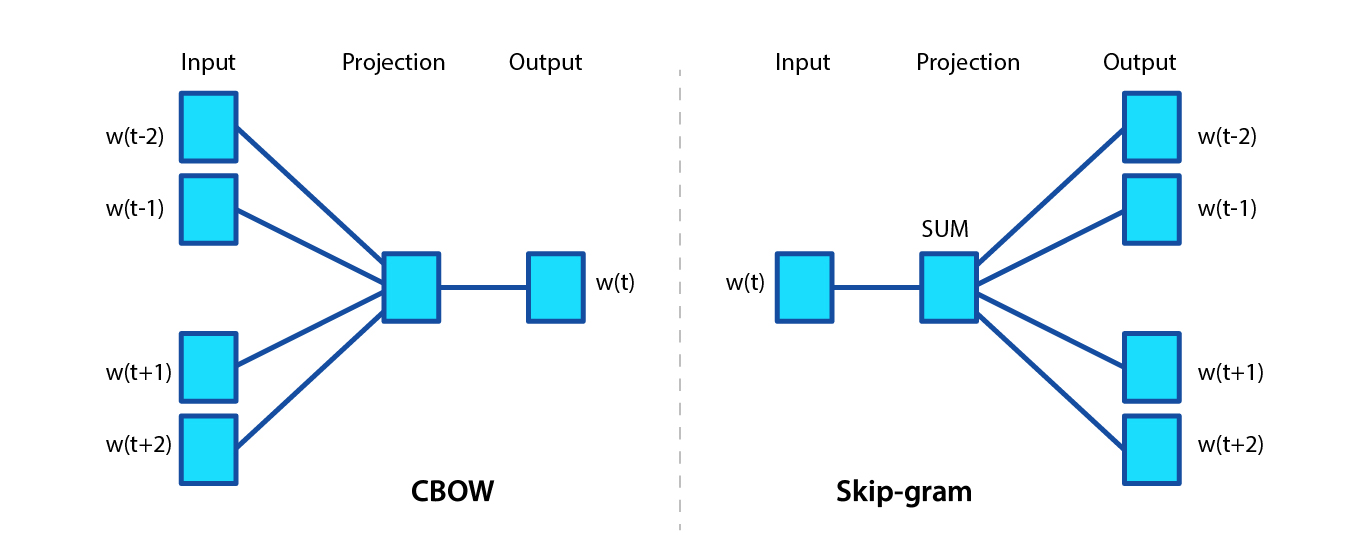
\includegraphics[keepaspectratio,
                     width=.8\paperwidth]{CBOW and skip-gram.jpg}
  \end{center}

  \noindent\rule{8cm}{0.4pt}

  {\footnotesize
  {\it Mikolov, Corrado, Chen, Dean} «Efficient Estimation of Word Representations in Vector Space», 2013}

\end{frame}


\begin{frame}
  \frametitle{Модель CBOW}

  Вероятность слова $w_t$ в заданном контексте $C_t = (w_{t-m}, \dots, w_{t-1}, w_{t+1}, \dots, , w_{t+m})$

  $$p(w_{t} = w|C_t) =    \underset{w \in W}{\text{SoftMax}} \left<u_w, v^{-t} \right> $$

  $v^{-t} = \frac{1}{2m} \sum\limits_{w \in C_t} v_w$ — средний вектор слов из контекста $C_t$

  $v_w$ — векторы предсказывающих слов,

  $u_w$ — вектор предсказываемого слова, в общем случае $u_w \neq v_w$

  \vspace{1cm}
  {\bf Критерий} максимума лог-правдоподобия, $U, V \in \mathbb{R}^{|W| \times d}$:

  $$ \sum\limits_{t=1}^n \log p(w_t|C_t) \to \max\limits_{U, V} $$

\end{frame}


\begin{frame}
  \frametitle{Skip-gram: как считать вероятности}

  \begin{columns}
      \begin{column}{.4\paperwidth}
        $ p(w_o|w_c) = \frac{\exp[v(w_o)u^T(w_c)]}{\sum\limits_{w=1}^W \exp[v(w)u^T(w_c)]}$

        $W$ — множество всех слов словаря

        $w_c$ — центральное слово

        $w_o$ — слово контекста

        $u(\cdot)$ и $v(\cdot)$ — вектора параметров (эмбединги), которые скалярно перемножаются
      \end{column}
      \begin{column}{.5\paperwidth}
        \begin{center}
          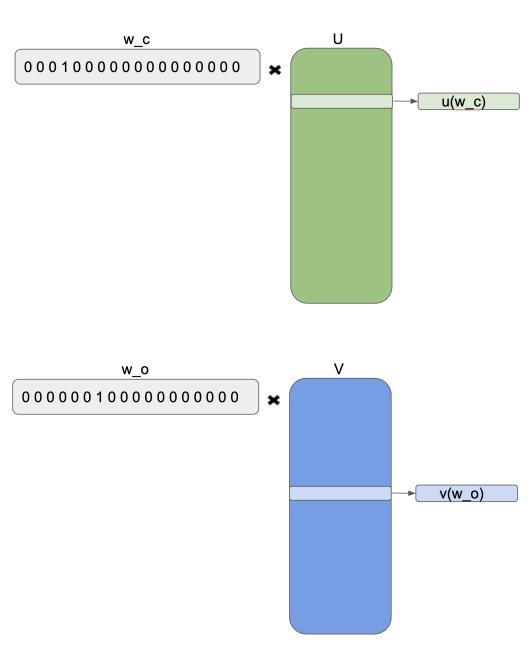
\includegraphics[keepaspectratio,
                           width=.5\paperwidth]{skip-gram-p.jpg}
        \end{center}
      \end{column}
  \end{columns}
\end{frame}


\begin{frame}
  \begin{question}
    В чем проблема такого подхода?
  \end{question}

  \pause
  В знаменателе, конечно, где все слова словаря.


  \pause
  \vspace{1cm}
  {\bf Mikolov} предложил
\end{frame}


\begin{frame}
  \frametitle{Иерархический софтмакс}
  Моделируем вероятность эффективнее. Строим дерево Хаффмана на словах, после чего:

  $1 - \sigma(x) = \sigma(-x)$

  $p(w_o|w_c) = \prod\limits_{n \in \text{Path}(w_o)} \sigma(d_{nw_o} v(n) u^T(w_c))$

  Здесь уже $v(n)$ — обучаемый вектор в узле дерева

  $d_{nw_o} = 1$, если $w_o$ в правом поддереве

  $d_{nw_o} = -1$ иначе

  \begin{center}
    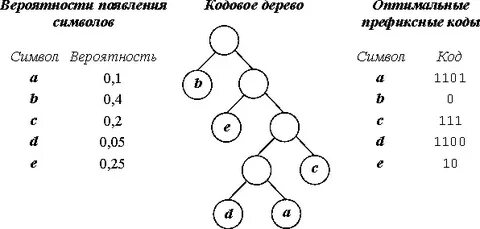
\includegraphics[keepaspectratio,
                     width=.5\paperwidth]{haffman.jpeg}
  \end{center}
\end{frame}


\begin{frame}
  \frametitle{doc2vec}
  \framesubtitle{на коленке}

  $$u^\prime (\text{doc}) = \sum\limits_{w \in \text{doc}} \omega_wu(w)$$

  \vspace{1cm}
  В качестве весов слов $\omega_w$ логично взять TF-IDF (term frequency / inverse document frequency)
\end{frame}


\begin{frame}
  \frametitle{Резюме}

  \begin{itemize}
    \item математическая постановка задачи тематического моделирования
    \item латентное размещение Дирихле (LDA)
    \item правдоподобие и перплексия языковой модели
    \item word2vec — модель получения векторных представлений слов
  \end{itemize}
  \pause
  \vspace{1cm}
  Что ещё можно посмотреть?
  \begin{itemize}
    \item \href{https://youtu.be/Eqm8-YqUzAc}{Лекция К.В. Воронцова про тематическое моделирование}
    \item \href{https://deeppavlov.ai/}{Open source фреймворк} для работы с текстами
  \end{itemize}
\end{frame}

\end{document}
